%%%%%%%%%%%%%%%%%%%%%%%%%%%%%%%%%%%%%%%%%%%%%%%%%%%%%%%%%%%%%%%%%%
%%%%%%%% ICML 2015 EXAMPLE LATEX SUBMISSION FILE %%%%%%%%%%%%%%%%%
%%%%%%%%%%%%%%%%%%%%%%%%%%%%%%%%%%%%%%%%%%%%%%%%%%%%%%%%%%%%%%%%%%

% Use the following line _only_ if you're still using LaTeX 2.09.
%\documentstyle[icml2015,epsf,natbib]{article}
% If you rely on Latex2e packages, like most moden people use this:
\documentclass{article}

% use Times
\usepackage{times}
% For figures
\usepackage{graphicx} % more modern
%\usepackage{epsfig} % less modern
\usepackage{subfigure} 

% For citations
\usepackage{natbib}

% For algorithms
\usepackage{algorithm}
\usepackage{algorithmic}

% As of 2011, we use the hyperref package to produce hyperlinks in the
% resulting PDF.  If this breaks your system, please commend out the
% following usepackage line and replace \usepackage{icml2015} with
% \usepackage[nohyperref]{icml2015} above.
\usepackage{hyperref}

% Packages hyperref and algorithmic misbehave sometimes.  We can fix
% this with the following command.
\newcommand{\theHalgorithm}{\arabic{algorithm}}

% Employ the following version of the ``usepackage'' statement for
% submitting the draft version of the paper for review.  This will set
% the note in the first column to ``Under review.  Do not distribute.''
%\usepackage{icml2015} 

% Employ this version of the ``usepackage'' statement after the paper has
% been accepted, when creating the final version.  This will set the
% note in the first column to ``Proceedings of the...''
\usepackage[accepted]{icml2015}
\usepackage[utf8]{inputenc}
\usepackage[T1]{fontenc}



% The \icmltitle you define below is probably too long as a header.
% Therefore, a short form for the running title is supplied here:
\icmltitlerunning{TP2 - Regressão Logistica}

\begin{document} 

\twocolumn[
\icmltitle{Machine Learning methods applied to soccer prediction}

% It is OKAY to include author information, even for blind
% submissions: the style file will automatically remove it for you
% unless you've provided the [accepted] option to the icml2015
% package.
\icmlauthor{Felipe Augusto Pereira Fernandes}{felipeapfernandes@gmail.com}
\icmladdress{CEFETMG}

% You may provide any keywords that you 
% find helpful for describing your paper; these are used to populate 
% the "keywords" metadata in the PDF but will not be shown in the document
\icmlkeywords{boring formatting information, machine learning, ICML}

\vskip 0.3in
]

\begin{abstract} 
Nesse relatório foi implementado o algoritmo de regressão logística na forma simples e multivariada. Esse relatório visa complementar os conhecimentos apresentados em sala de aula.
\end{abstract} 

\section{Introduction}
Soccer is the most popular sport in the world \cite{FIFA}. Its popularity can be assigned to its simplicity, because only something that characterize the goal and the ball is needed to its practice. Soccer is also a subject always present on pubs tables, family and friends reunions. Who is going to win the league? Which team is better? are question raised on these talks. This is the reason that nowadays communication vehicles, like TV shows, have now specialists to discuss and make projections about which team is going to win the league or the round's fixture outcome.

Determine the outcome of a match is not a simple task, because soccer is a collective game subject to inumerous variables, such as team pattern, tactic scheme, formation, individuals failures, player's skills, team motivation, referees's decisions \textit{etc}.

Statistics of game, teams and players are used to aid the determine soccer matches's outcome. Nowadays, these statistics are being used on soccer transmission to demonstrate better the scenario of a match, avoiding the subjectivity.

Looking into a team, it is possible to establish a performance history along the season. With the help of these statistics numbers such as number of goals per
match, percentage of complete passes per game, it is possible to establish features that could describe a soccer match. 

With the aid of Machine Learning methods, this study aims to investigate the impact of features into  soccer prediction, using a public database of matches. This database contains more than 25000 matches from 8 different leagues across 8 seasons. This database was published in August 2016 on Kaggle website \cite{kaggledatabase}.

This study aims to elaborate input models for multilayer perceptron networks
with basic performance data, like number of victories, losses, draws, goals
scored and goals suffered.
		
		\begin{figure}[ht]
			\vskip 0.2in
			\begin{center}
				\centerline{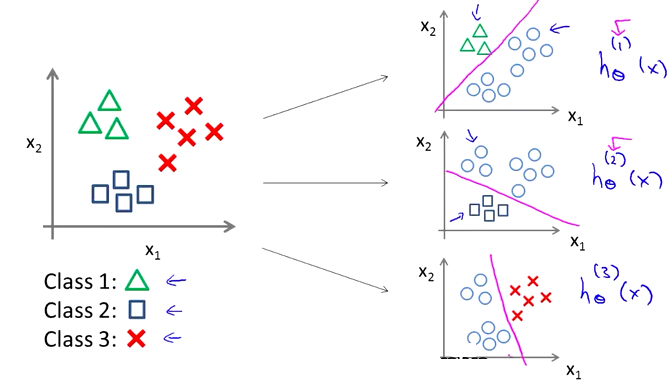
\includegraphics[width=\columnwidth]{img/onevsall.jpg}}
				\caption{Demonstração: One vs all Fonte: Stanford University - ML Class}
				\label{fig:onevsall}
			\end{center}
			\vskip -0.2in
			
		\end{figure}
	
	
	\begin{thebibliography}{8}
		\bibitem{aslan2007comparative}
		ASLAN, B. G.; INCEOGLU, M. M. A comparative study on neural network based soccer
		result prediction. In: IEEE. \emph{Intelligent Systems Design and Applications, 2007. ISDA
			2007. Seventh International Conference on.} [S.l.], 2007. p. 545–550.
		\bibitem{cheng2003new}
		CHENG, T.; CUI, D.; FAN, Z.; ZHOU, J.; LU, S. A new model to forecast the results of matches based on hybrid neural networks in the soccer rating system. In: IEEE. \emph{Computational Intelligence and Multimedia Applications, 2003. ICCIMA 2003. Proceedings. Fifth International Conference on.} [S.l.], 2003. p. 308–313.
		\bibitem{matrixConf}
		CONGALTON, R. G. \emph{A review of assessing the accuracy classifications of
			remotely sensed data}. Remote Sensing of Environment, New York, v. 49, n. 12, p.
		1671-1678, Dec. 1991.
		\bibitem{Elo}
		Elo, A.E.: \emph{The Rating of Chess Players, Past and Present}, Arco Publishing, New York (1978).
		\bibitem{FIFA}
		FIFA. 270 million people active in football. \emph{FIFA Communications Division, Information Services,} v. 31, p. 2007, 2006.
		\bibitem{ingles}
		O Gol, \emph{www.ogol.com.br :: Tudo sobre Futebol}, http://www.ogol.com.br, acessado em 14 de maio de 2015.
		\bibitem{sofifa}
		SoFIFA, \emph{Teams - FIFA - SoFIFA}, http://sofifa.com/teams/?hl=en-GB, acessado em 14 de maio de 2015.
		
		\bibitem{Haykin}
		S. O. Haykin, \emph{Neural Networks and Learning Machines}. Prentice-Hall, 2008.
		%\verb+\+hskip 1em plus 0.5em minus 0.4em\verb+\+relax
	\end{thebibliography}
		
\end{document} 



